\chapter{Análisis}
\section{Análisis de Requerimientos}
Este proyecto permite que los usuarios llevar a cabo transacciones con el fin de compartir información pertinente para el manejo de lo que sea de la empresa...

La interacción de los usuarios con los sistemas construidos se presenta en la Figura \ref{fig:Analisis}, la cual describe los siguientes pasos. 1) El analista hace xyz. 2) El Cliente responde ABC...

\begin{figure}[ht] 
\centering
\caption{Diagrama de contexto}
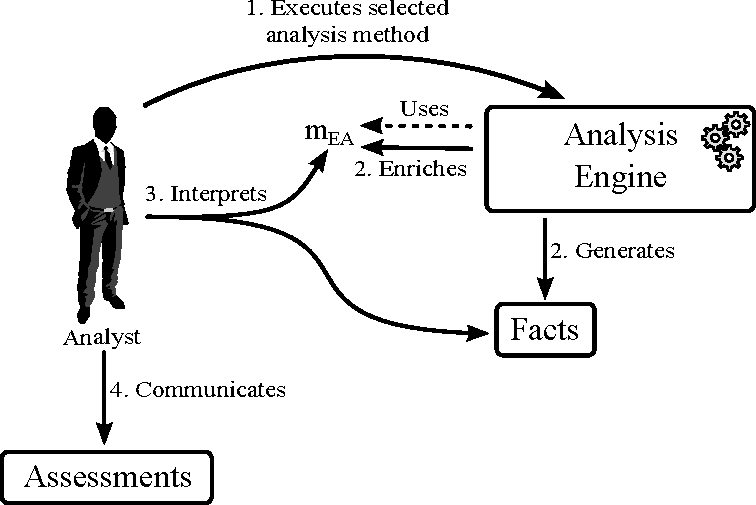
\includegraphics[width=0.6\textwidth]{img/analisis.pdf}
\label{fig:Analisis}  
\end{figure} 

El diagrama de procesos se presenta en la Figura \ref{fig:Diagrama-de-Procesos}. En diagrama presenta las actividades que el proyecto incluye...

\begin{figure}[ht] 
\centering
\caption{Diagrama de Procesos}
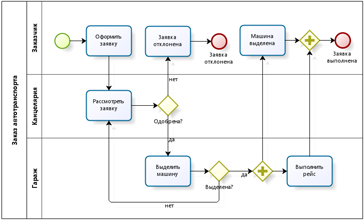
\includegraphics[width=0.5\textwidth]{img/bpmn.png}
\label{fig:Diagrama-de-Procesos}  
\end{figure} 

\subsection{Requerimientos}

\begin{enumerate}

\item Ingreso:
\begin{itemize}
    \item Ingreso con correo y contraseña
    \item Registro
    \item Recuperacion de contraseña
\end{itemize}

\item Facturación:
\begin{itemize}
    \item Ingreso de codigo
    \item Busqueda de productos
    \item Tabla de items facturados
    \item Subtotal
    \item IVA
    \item Total
\end{itemize}

\item Inventario:
\begin{itemize}
    \item Filtro por fechas
    \item Exportar con formato .CSV
\end{itemize}

\end{enumerate} 

\subsection{Requerimientos Funcionales}
Los requerimientos funcionales describen los diferentes servicios que el proyecto debe proveer... La Tabla \ref{table:Requerimientos-Funcionales} presenta los requerimientos funcionales del sistema.

\begin{center}
\begin{longtable}{p{3cm} p{12cm}}
\caption{Requerimientos Funcionales}
\label{table:Requerimientos-Funcionales}
\\ \hline \hline

\textbf{ID} & \textbf{RF 01} \\ \hline
\textbf{Nombre} & Sistema Administrador De Directores \\ \hline
\textbf{Descripción} & El usuario administrador crea el nuevo usuario director para la administración de categorías y productos. Debe llenar los campos de nombre, apellido, contraseña, email, teléfono y contraseña. El id del director se asigna automáticamente.  \\ \hline
\textbf{Actores} & Administrador \\ \hline
\textbf{Observaciones} & El usuario administrador tiene la opción de agregar, consultar, editar, habilitar y deshabilitar a los directores creados. \\ \hline
\hline \\ \hline \hline

\textbf{ID} & \textbf{RF 02} \\ \hline
\textbf{Nombre} & Sistema Administrador De Categorías \\ \hline
\textbf{Descripción} & El usuario director gestiona categorías. Debe llenar los campos de nombre, descripción, estado (activo o inactivo). El id de la categoría se asigna automáticamente al igual que el id del director autenticado en ese momento.  \\ \hline
\textbf{Actores} & Director \\ \hline
\textbf{Observaciones} & El usuario director tiene el control para realizar las acciones de crear, consultar, editar, habilitar y deshabilitar las categorías de la tienda. \\ \hline
\hline \\ \hline \hline

\textbf{ID} & \textbf{RF 03} \\ \hline
\textbf{Nombre} & Sistema Administrador De Productos \\ \hline
\textbf{Descripción} & El usuario director asigna productos por categoría. Debe llenar los campos de nombre, descripción, precio de oferta, precio original, estado (activo o inactivo). Se debe seleccionar también una categoría para el producto. El id del producto se asigna automáticamente.  \\ \hline
\textbf{Actores} & Director \\ \hline
\textbf{Observaciones} & El usuario director tiene la opción para crear, consultar, editar, habilitar y deshabilitar los productos de las categorías. \\ \hline
\hline
\end{longtable}
\end{center}

\subsection{Requerimientos No Funcionales}
Los requerimientos no funcionales describen diferentes caracteristicas adicionales que el proyecto debe satisfacer para poder llevar a cabo los servicios que provee... La Tabla \ref{table:Requerimientos-No-Funcionales} presenta los requerimientos no funcionales.

\begin{center}
\begin{longtable}{p{3cm} p{12cm}}
\caption{Requerimientos No Funcionales}
\label{table:Requerimientos-No-Funcionales}
\\ \hline \hline

\textbf{ID} & \textbf{RNF 01} \\ \hline
\textbf{Nombre} & Hosting \\ \hline
\textbf{Descripción} & Características de Dreamhost, hosting en el cual se alojan el sistema web y base de datos.  \\ \hline
\textbf{Observaciones} & Servidor de 2 núcleos de CPU, 4GB RAM disponible, almacenamiento de 60GB SAN, ancho de banda de 2 TB, 2 IPs disponibles \\ \hline 
\hline \\ \hline \hline

\textbf{ID} & \textbf{RNF 02} \\ \hline
\textbf{Nombre} & Concurrencia \\ \hline
\textbf{Descripción} & El sistema deberá soportar una concurrencia del 20 por ciento de usuarios (sobre una base de 300 usuarios), donde los tiempos de respuesta se mantienen.  Con un valor mayor de concurrencia el sistema sigue prestando servicio pero los tiempos de respuesta empiezan a aumentar. La concurrencia estará dada en los puntos donde se realizan consulta y carga de información en el sistema. \\ \hline
\hline \\ \hline \hline

\textbf{ID} & \textbf{RNF 03} \\ \hline
\textbf{Nombre} & Navegadores \\ \hline
\textbf{Descripción} & El sistema debe estar conectado a internet y los navegadores actualizados. \\ \hline
\textbf{Observaciones} & Navegador Mozilla Firefox versión 3.6 o superior, navegador Internet Explorer versión 8.0 o superior, navegador Chrome Version 36 o superior y velocidad de internet desde 2MB \\ \hline
\hline \\ \hline \hline

\textbf{ID} & \textbf{RNF 04} \\ \hline
\textbf{Nombre} & Disponibilidad \\ \hline
\textbf{Descripción} & El sistema y aplicación está disponible para el ingreso y consulta de los usuarios. Se requiere que el sistema tenga una disponibilidad general del 97 por ciento por año. Esto quiere decir que el sistema podrá estar caído máximo 262 horas durante el año \\ \hline
\textbf{Observaciones} & El sistema requiere una disponibilidad del 97 por ciento para el periodo diario completo, en el horario de 24x7.  Esto quiere decir que el sistema sólo podrá estar caído máximo 0,3 horas (18 minutos) dentro de dicho periodo, sin contabilizar el tiempo de reinicialización de las máquinas. La disponibilidad del sistema dependerá de la disponibilidad del proveedor de acceso a Internet o de los servicios de interconexión prestados por terceros. \\ \hline 
\hline

\end{longtable}
\end{center}

\section{Definición de Actores}
Con base en el análisis de requerimientos realizado, se establecen los actores que se presentan en la Tabla \ref{table:Actores}. 

\begin{center}
\begin{longtable}{p{2.5cm} p{12cm}}
\caption{Actores}
\label{table:Actores}
\\ \hline \hline

\textbf{Nombre} & \textbf{Administrador} \\ \hline
\textbf{Descripción} & Actor encargado de gestionar todo lo relacionado con la gestión de usuarios directores. Además, puede modificar cualquier dato del sistema \\ \hline
\textbf{Atributos} & Nombre, apellido, identificación, contraseña, fecha de vinculación \\ \hline \hline
\hline \\ \hline \hline

\textbf{Nombre} & \textbf{Director} \\ \hline
\textbf{Descripción} & Actor encargado de gestionar todo lo relacionado con la gestión de categorías y productos. \\ \hline
\textbf{Atributos} & Nombre, apellido, identificación, contraseña, fecha de vinculación \\ \hline \hline
\hline \\ \hline \hline

\textbf{Nombre} & \textbf{Cliente} \\ \hline
\textbf{Descripción} & Actor final de la aplicación, gestiona todo lo relacionado con el proceso de pedidos. \\ \hline
\textbf{Atributos} & Nombre, apellido, identificación, contraseña, fecha de vinculación \\ \hline \hline
\hline

\end{longtable}
\end{center}